\section{Orthogonal Tensor Trains}\label{sec:ott}
As described in Chapter~\ref{chap:bknd}, a number of TT operations with respect to approximation and projection require computing the QR decomposition of matricized cores. In the applications for which tensor trains were originally developed, these operations were necessary \citep{oseledets2011tensor,klus2018tensor}. For modern neural network applications, where the tensor operator may be our target of learning, it may be sufficient to treat each matrix product as its own variable, and through the standard TT decomposition learn the cores along the \textbf{product of Stiefels}.

A na\"ive approach may orthogonalize the reshaped cores, and progressively push the upper triangular part of the core decomposition into the next core, resulting in the following exact formulation with appropriate reshaping:
\begin{align}
%    X(x_1,\ldots,x_d) &= A_1(x_1)\cdots A_d(x_d) \\
    \cX &= A_1^L A_2^L\cdots A_d^L \nonumber\\
    &= Q_1^L R_1 A_2^L \cdots A_d^L = Q_1^L \left(R_1 A_2^L\right) \cdots A_d^L \nonumber\\ 
    &= Q_1^L Q_2^L R_2 \cdots A_d^L \nonumber\\
    &= Q_1^L \cdots Q_d^L R_d \label{eq:eott}
\end{align}
where $ [Q_1^L, R_1] = qr(A_1^L) $, $ [Q_i^L, R_i] = qr(R_{i-1} A_i^L ), \ i \in \left \{2,\ldots,d \right \}$, and $ Q_i^L \in \RR^{r_{i-1} n_i \times r_i}$ with $R_i \in \RR^{r_i \times r_i}$. 
Each $Q_i^L$ is on a Stiefel given by $\ST(r_i, r_{i-1}n_i)$. Here, the number of components in the product space of Stiefels is $d$, with the `residual' $R_d \in \RR$. This decomposition is exact and only requires a reshaping of the tensor cores.
If all $r_i = r, n_i = n$,
then the total number of parameters needed is
 % the number of parameters becomes 
%is $ d n r^2 - (d-1)\frac{r^2 + r}{2}$,
%\begin{align*}
%    &=\sum_{i=1}^d \left[nr^2 - \frac{r(r + 1)}{2}\right] + \frac{r(r+1)}{2} \\
%    &= d n r^2 - d\frac{r(r + 1)}{2} + \frac{r(r+1)}{2} \\
$    d n r^2 - (d-1)\frac{r^2 + r}{2},$
%\end{align*}
%\begin{align}
%    \sum_{i=1}^d \left[r_{i-1}n_i r_i - \frac{r_i(r_i + 1)}{2}\right] + \frac{r_d(r_d+1)}{2}
%\end{align}
compared to the full format with $dnr^2$ total parameters.
It is important to note that in this formulation, the cores themselves are \textbf{not} orthogonal. Reshaping is required to bring the matricized form back to TT-cores of size $r_{i-1} \times r_i$, and in practice it is not easy to perform simple TT-tensor multiplication in this form. Additionally, we now need to optimize over Stiefel manifolds of a larger size, namely $O(nr^2)$.

\subsection{A Nicer Tensor Train Approximation}
Ideally, we would prefer a construction which keeps the standard TT-core format and involves optimization over ``smaller'' Stiefel manifolds. Consider the following representation, in which each TT-core itself is orthogonal.
\begin{definition}\label{def:ott}(Orthogonal Tensor Train)
The Orthogonal Tensor Train is defined as
\begin{align}
\cX(x_1,\ldots,x_d) = Q_1(x_1) \cdots Q_d(x_d),
\end{align}
where each $Q_i(x_i)$ lies on the Stiefel $\ST(m_i, M_i)$, and $m_i = \min(r_{i-1},r_i)$, $\ M_i = \max(r_{i-1},r_i)$.
\end{definition}
While in this formulation the total number of components in the product space of Stiefels is $nd$, the dimension of each manifold is \textbf{significantly smaller},
dependent {\em only} on the core rank as opposed to the mode size.
The total number of parameters, if $n_i =n, r_i = r$, is
\begin{align}
n \sum_{i=1}^d \left[ r^2 - \frac{r^2 + r}{2}\right] = d n r^2 - dn\frac{r^2 + r}{2}.
\end{align}
When compared to the full TT representation,
the Orthogonal Tensor Decomposition (OTT) requires
$(r+1)/2r \approx 1/2$ as many parameters.
If $r_i=r_{i+1}$, then $\ST(m_i, M_i) = SO(m_i)$, where $SO$ is the special orthogonal group.

This construction can be seen as an approximation to the full tensor train format, in which the upper triangular part of each core is set to identity:
\begin{align}
    &\cX(x_1,\ldots,x_d) = A_1(x_1)\cdots A_d(x_d) \nonumber\\ &= Q_1(x_1)R_1(x_1)\cdots Q_d(x_d)R_d(X_d) \nonumber\\
    &\approx Q_1(x_1) \cdots Q_d(x_d)
    %&= \sum_{r_0}\cdots\sum_{r_d} A_1(x_1)[r_0,r_1]\cdots A_d(x_d)[r_{d-1},r_d] \\
\end{align}

%\begin{remark}
\paragraph{Is this useful?} It is not obvious that this construction is useful at all. How much is lost through this approximation? What is gained by using this construction? In what follows, we demonstrate that we can approximate any tensor with bounded norm using an OTT, and that with a full rank assumption and a trainable constant, our formulation admits a solution with $\epsilon$ error.
\begin{algorithm}
	\caption{Stochastic OTT Optimization}\label{alg:ott_opt}
	\SetAlgoLined
	\DontPrintSemicolon
	\For{t=1,\ldots,T}{
		$g_t := \frac{df}{d\cW} f(X^{mini-batch})$\\
		\For{\text{Core} $Q^i_t \in \cW_t$ \text{and Core Gradient} $g^i_t \in g_t$}{
			$G^i_t = P_{T_{\cW_t}M}(g^i_t)$ \Comment*[r]{Projection Step}
			$Q^i_{t+1} \leftarrow \Exp(Q^i_t, G^i_t)$ \Comment*[r]{Retraction Step}
		}
	}
\end{algorithm}
\begin{figure}
	\centering
	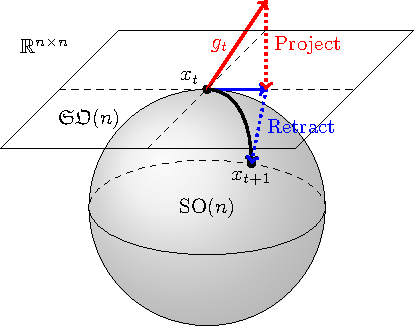
\includegraphics[width=0.75\columnwidth,trim={0 1.5cm 0 0},clip]{4_ott/figs/stiefel/stiefel_update.pdf}
	\caption{\label{fig:ott_opt} Gradient descent algorithm using the projection and retraction on the Stiefel manifold. The update is applied to each core individually, allowing for smaller manifold operations that would otherwise scale poorly with dimension.}
\end{figure}

\subsection{Theoretical Analysis}
We start by reshaping any tensor $\cX$ to a matrix $X^M$ by grouping the modes into two groups, $X^M \in \RR^{n \times m}$. We may fix this arbitrary matrix as $X^M = A \in \RR^{n \times m}$.

\begin{proposition}
\label{theory:prop1}
Given a 2D tensor $A\in \RR^{m\times m}$, $A_{ij} \in [-1,1]$, there exists sets of unit vectors, $\left\{\mathbf{x}_i\right\}_{i=1}^m\subset \RR^m$, $\left\{\mathbf{y}_j\right\}_{j=1}^m\subset \RR^m$ such that, $\forall \epsilon > 0$, $\|A - \widetilde{A}\| < \epsilon$, where, $\forall i,j,\: \widetilde{A}_{ij}=\mathbf{x}_i^t\mathbf{y}_j$.
\end{proposition}
\begin{proof}
  Let $A=USV^T$ be the SVD of $A$. Let $\epsilon > 0$, we will perturb $S$ along the diagonal to generate $\widetilde{S}$ such that, $\|S - \widetilde{S}\| < \epsilon$. Let $X=\left[\mathbf{x}_i\right]$ and $Y=\left[\mathbf{y}_i\right]$. We will first give an algorithm to generate $\widetilde{X}$ and $\widetilde{Y}$ with each
  of its column being orthonormal such that, $\widetilde{X}^T\widetilde{Y}=S$. Then, $X=\widetilde{X}U^T$ and $Y=\widetilde{Y}V^T$. 

We begin with an algorithm for $m=3$. Choose $\left\{\widetilde{\mathbf{x}}_i\right\}$ to be unit vectors and assign $\widetilde{\mathbf{y}}_3=\widetilde{\mathbf{x}}_1\times \widetilde{\mathbf{x}}_2$, $\widetilde{\mathbf{y}}_2=\widetilde{\mathbf{x}}_3\times \widetilde{\mathbf{x}}_1$. Then, make $\widetilde{\mathbf{y}}_2$ and $\widetilde{\mathbf{y}}_3$ to be of unit length. %Clearly, $\widetilde{\mathbf{x}}_2^t\widetilde{\mathbf{y}}_2\neq 0$ and $\widetilde{\mathbf{x}}_3^t\widetilde{\mathbf{y}}_3\neq 0$. 
Now, rotate $\widetilde{\mathbf{x}}_2$ in the plane spanned by $\left\{\widetilde{\mathbf{x}}_1, \widetilde{\mathbf{x}}_2\right\}$ such that,
$\widetilde{\mathbf{x}}_2^t\widetilde{\mathbf{y}}_2=\widetilde{S}_{22}$. Similarly, rotate $\widetilde{\mathbf{x}}_3$ in the plane spanned by $\left\{\widetilde{\mathbf{x}}_3, \widetilde{\mathbf{x}}_1\right\}$ such that,
$\widetilde{\mathbf{x}}_3^t\widetilde{\mathbf{y}}_3=\widetilde{S}_{33}$. Now, assign, $\widetilde{\mathbf{y}}_1=\widetilde{\mathbf{x}}_2\times \widetilde{\mathbf{x}}_3$ and make it unit length. Now, fixing $\widetilde{\mathbf{x}}_2$ and $\widetilde{\mathbf{x}}_3$, the above steps are a continuous mapping, $F$ from $\mathbf{S}^2$ to $[-1,1]$, i.e., by changing different $\widetilde{\mathbf{x}}_1 \in \mathbf{S}^2$, we will get different values for $\widetilde{\mathbf{x}}_1^t\widetilde{\mathbf{y}}_1$. Also, notice that, if, for a particular choice of $\left\{\widetilde{\mathbf{x}}_i\right\}$, $\widetilde{\mathbf{x}}_1^t\widetilde{\mathbf{y}}_1>0$, then, for the choice of $\left\{\widetilde{-\mathbf{x}}_i\right\}$, the above construction returns $-\widetilde{\mathbf{y}}_2$ and $-\widetilde{\mathbf{y}}_3$ and $F$ returns, $-\widetilde{\mathbf{x}}_1^t\widetilde{\mathbf{y}}_1<0$. Thus if $a \in F\left(\mathbf{S}^2\right)$,  $-a \in F\left(\mathbf{S}^2\right)$. Furthermore, $1\in F\left(\mathbf{S}^2\right)$ and hence, $-1\in F\left(\mathbf{S}^2\right)$. As $\mathbf{S}^2$ is connected and $F$ is continuous,
$F\left(\mathbf{S}^2\right)$ is connected, and so, $\exists$ $\left\{\mathbf{x}_i\right\}_{i=1}^m\subset \RR^m$ and $\left\{\mathbf{y}_j\right\}_{j=1}^m\subset \RR^m$, s.t., $\left(\forall \left\{i, j\right\}\right)$, 
$\widetilde{\mathbf{x}}_i^t\widetilde{\mathbf{y}}_j = \widetilde{S}_{ij}$. Since $\|S-\widetilde{S}\|< \epsilon$ and the
choice of $\epsilon> 0$ is arbitrary, we can see that $\|A - \widetilde{A}\| < \epsilon$.

Using the generalization of cross product by exterior algebra, the above procedure can be naturally extended to arbitrary $m>3$.
\end{proof}

A direct corollary of the above result allows approximating an arbitrary 2D matrix,
\begin{corollary}\label{theory:corr1}
Given a 2D tensor $A \in \RR^{m \times m}$, there exists sets of unit vectors, $\left\{\mathbf{x}_i\right\}_{i=1}^m\subset \RR^m$, $\left\{\mathbf{y}_j\right\}_{j=1}^m\subset \RR^m$ and fixed constant $c$ such that, $\forall \epsilon > 0$, $\|A-\widetilde{A}\|< \epsilon$, where, $\forall i,j,\: \widetilde{A}_{ij}=c\mathbf{x}_i^t\mathbf{y}_j$.
\end{corollary}
\begin{proof}
Given any arbitrary matrix $A$, define $A^\prime = A/|A|_{\infty}$. Then $A^\prime_{ij} \in [-1,1]$, and by Proposition \ref{theory:prop1} we can construct unit vectors $\textbf{x}_i,\textbf{y}_j$ such that $\forall \epsilon > 0$, $\|A^\prime_{ij} - \textbf{x}_i^T\textbf{y}_j\|< \epsilon$. Then immediately $\forall A_{ij}$, we have $A_{ij} = cA^\prime_{ij}$ where $c = |A|_\infty$.
\end{proof}

We also have the following directly from Proposition \ref{theory:prop1}.
%%%%%%%%%%% matrix vector
\begin{corollary}\label{theory:corr2}
Given a 2D tensor $A\in \RR^{m\times m}$, with $\|A\|_F\leq 1$, there exists a set of orthonormal matrices $\left\{B_i\right\} \subset SO(m)$ and a set of unit vectors $\left\{\mathbf{y}_j\right\}_{i=1}^m\subset \RR^m$ such that $\forall \epsilon > 0$, $\|A - \widetilde{A}\|< \epsilon$, where, $\forall i,j,\: \widetilde{A}_{ij}= \mathbf{1}^t B_i^t\mathbf{y}_j$.
\end{corollary}
%\begin{proof}
%The proof follows from Proposition \ref{theory:prop1}.
%\end{proof}

\begin{example}Applying the above result to OTT, equivalence is relatively straightforward to show. 
%\begin{example}
Consider the problem of approximating a 4 dimensional tensor $\cX$ with $n_{1,2,3,4}=n=r$. Let $Q_1(x_1) \in \RR^{1\times n}, Q_2(x_2), Q_3(x_3) \in \RR^{n \times n}$, and $Q_4(x_4) \in \RR^{n \times 1}$. By Corollary \ref{theory:corr2} we can write two vectors indexed by $x_1,x_2$ and $x_3,x_4$ as $X^A (x_1,x_2) = Q_1(x_1)^\top Q_2(x_2)$ and  $X^B(x_3,x_4) = Q_3(x_3)Q_4(x_4)$ respectively. The multiplication of these vectors $X^A,X^B$ again yields a single element indexed by $x_1,x_2,x_3,x_4$, which can take any value between $[-1,1]$ by Proposition \ref{theory:prop1}. Then clearly the cores $Q$ form an equivalent definition of $\cX$.
%\end{example}
\end{example}

We can then apply Corollary \ref{theory:corr2} and find that the product of indexed orthonormal matrices and orthonormal vectors with full rank can approximate any matrix with bounded norm. 
Applying this to our OTT format, it immediately follows that with  the addition of at most $dn$ constants in $\RR$ we can approximate any arbitrary tensor. While this addition would put the format well over the number of parameters in the standard format, this provides sufficient evidence that, in typical learning settings in which our model is already overparameterized, we can still capture the full expressive power of the model class in which an OTT format is inserted. 

\paragraph{Remark.} It also important to note that the above calculation of dimensionality is the \textit{intrinsic} dimension. The number of actual allocated variables is indeed $dn^3$ for an exact formulation.
It remains open to theoretically analyze the degradation of the approximation as $r<n$.

\subsection{Efficient Stiefel Optimization}\label{sec:opt}
Here, we describe how to compute an OTT approximation of a tensor $\cW$, which can be posed as the following minimization problem.
\vspace{-5pt}
\begin{align}
\min_{\left\{Q_i(x_i)\right\}_{i=1}^d} E &= \sum_{\left\{x_i\right\}} \|\cW(x_1,\ldots,x_d) - Q_1(x_1)\cdots Q_d(x_d)\| \notag \\ \quad & \mbox{s.t.} \quad Q_i(x_i)^\top Q_i(x_i) = I_p \quad \forall i, x_i
\end{align}
Notice that this optimization is difficult because of the orthogonality constraint \cite{edelman1998geometry,collins2014spectral}. An efficient way to solve this is by doing the optimization on the product of (compact) Stiefel manifolds: let it be denoted by $\mathcal{P}_S$. We will use the product $\ell_2$ metric on this product space. Given $x_1, \cdots x_d$, we perform
an optimization on the product of Stiefel manifolds to solve for $\{Q_i(x_i)\}$ for $i\in[1\ldots d]$. We use a Riemannian gradient descent technique on this product of Stiefel manifolds $\mathcal{P}_S$. Given $\{Q^t_i(x_i)\}$ as the solution of the $t^{th}$ step, the $(t+1)^{th}$ solution, $\{Q^{t+1}_i(x_i)\}$, can be computed using 
\vspace{-5pt}
\begin{equation}
\left\{Q^{t+1}_i(x_i)\right\} = \text{Exp}\left(\left\{Q^{t}_i(x_i)\right\}, \frac{\partial E}{\partial \left\{Q^{t}_j(x_j)\right\}}\right),
\end{equation}
where $\text{Exp}$ is the Riemannian Exponential map on $\mathcal{P}_S$. On $\mathcal{P}_S$, computation of Riemannian Exponential map is not tractable and needs an optimization, hence we
use a Riemannian retraction map as proposed in \cite{6340355}.

Figure \ref{fig:ott_opt} summarizes this procedure. For each orthogonal core, the gradient is computed with respect to the Euclidean ambient space and projected to the tangent space at the current iterate. The update is constructed by moving back to the Stiefel with the Riemannian exponential map.

\subsection{Square Stiefels/SO(n)}
In practice, when learning an OTT operator, we will primarily be setting the rank to be fixed for all cores.
The Stiefel manifold, $\ST(n,n)$ with $n=p$ is equal to the special orthogonal group $\text{SO}(n)$.
The Riemannian Exponential map on $\text{SO}(n)$ is the matrix exponential, computationally intensive to both compute and backpropagate through.
Hence, we use the Cayley map from $\mathfrak{SO}(n)$ to $\text{SO}(n)$, given by $A \mapsto \left(I-A\right)\left(I+A\right)^{-1}$, where $\mathfrak{SO}(n)$ (the space of $n\times n$ skew-symmetric matrices) is the tangent space of $\text{SO}(n)$ at identity.
Although the Cayley map requires a matrix inverse, it is much easier to handle using standard tools
in modern toolboxes (e.g., TensorFlow, PyTorch).
%\begin{algorithm}
%	\caption{OTT Core.}\label{alg:ott-core}
%	\SetAlgoLined
%	\DontPrintSemicolon
%	\SetKwFunction{FMain}{OTT-Core}
%	\SetKwProg{Fn}{Function}{:}{}
%	\Fn{\FMain{$r$}}{
%		$w \leftarrow \RR^{r(r-1)/2}$ \\
%		$R \leftarrow \text{triu}(w)$ \\
%		$A \leftarrow R - R^\top$ \\
%		$Q \leftarrow (I - A)(I + A)^{-1}$ \\
%		\KwRet{$Q$}
%	}
%\end{algorithm}
Observe that
the work in \cite{helfrich2017orthogonal} used the Cayley map for RNNs, but does not make use of the sparse representation of a skew-symmetric matrix $A \in \mathfrak{SO}(n)$.
In contrast, in our formulation we use the Cayley map as a mapping from $\mathbb{R}^{\frac{n(n-1)}{2}}$ to $\text{SO}(n)$. This enables a strict reduction in the number of trainable/learnable variables in a network, and provides a direct path through which gradients can be computed and backpropagated.
Algorithm \ref{alg:ott-core} describes the procedure for constructing an OTT-core.
The Euclidean variable vector $w$ is mapped directly to the upper triangular part, defined as $\triu(\cdot)$, of a new matrix $R$, and by subtracting its transpose,
we arrive at a skew symmetric matrix $A$. The Cayley map, as described above, maps to our Orthogonal OTT Core. 

\paragraph{Remark.} Note that the Cayley map is not a bijective mapping between $\mathfrak{SO}(n)$ and $\text{SO}(n)$ as the range is not the entire $\text{SO}(n)$. This is because the Cayley map cannot generate matrices with negative eigenvalue(s). Empirically, we do not find this to be an issue when learning the OTT representation directly.

With this efficient approximation in hand, we are able to directly apply our OTT formulation to architectures for a variety of applications.
\begin{algorithm}
	\caption{ \label{alg:ott-core} Constructing an OTT Variable}
	\SetAlgoLined
	\DontPrintSemicolon
	\SetKwFunction{FVar}{OTT-Variable}
	\SetKwProg{Fn}{Function}{:}{}
	\Fn{\FVar{$d, n_{in}, n_{out}, r$}}{
       $OTT \leftarrow \emptyset$ \\
       \For{$i \in 1,\ldots,d$}{
           \For{$j,k \in 1,\ldots,n_{in}[i],1,\ldots,n_{out}[i]$}{
                $OTT$.append(OTT-Core($r$)) \\
			}
       }
		\KwRet{$OTT$}
	}
	\SetKwFunction{FCore}{OTT-Core}
	\SetKwProg{Gn}{Function}{:}{}
	\Gn{\FCore{$r$}}{
		$w \leftarrow \RR^{r(r-1)/2}$ \\
		$R \leftarrow \text{triu}(w)$ \\
		$A \leftarrow R - R^\top$ \\
		$Q \leftarrow (I - A)(I + A)^{-1}$ \\
		\KwRet{$Q$}
	}
\end{algorithm}